\section{Vizuelizacija}
\label{sec:Vizuelizacija}
Kako bi se razumeli rezultati istra\v{z}ivanja, izvr\v{s}ena je njihova vizuelizacija. Na slici \ref{fig:Geolokacija} prikazana je zastupljenost autora na razli\v{c}itim lokacijama. Ova informacija je kori\v{s}\'c{}ena u odeljku \ref{Genre-Location}.

\begin{figure}[h]
    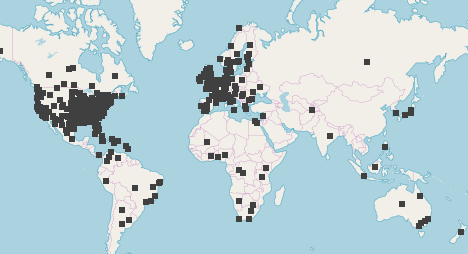
\includegraphics[scale=0.45]{resources/Geolokacija.png}
    \label{fig:Geolokacija}
    \caption{TODO name}
\end{figure}


Zastupljenost \v{z}anrova je prikazana na \ref{fig:ZastupljenostZanrova}.
\begin{figure}[h]
    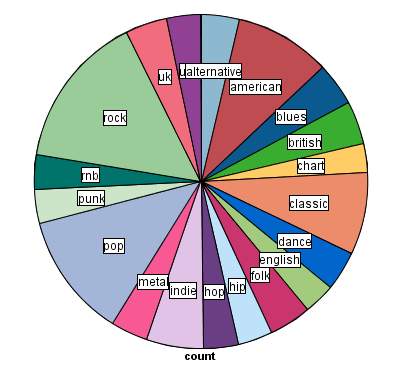
\includegraphics[scale=0.6]{resources/ZastupljenostZanrova.png}
    \label{fig:ZastupljenostZanrova}
    \caption{Zastupljenost \v{z}anrova}
\end{figure}


Zavisnost du\v{z}ine pesama u odnosu na godinu nastanka prikazana je na \ref{fig:YearDuration}.
\begin{figure}[h]
    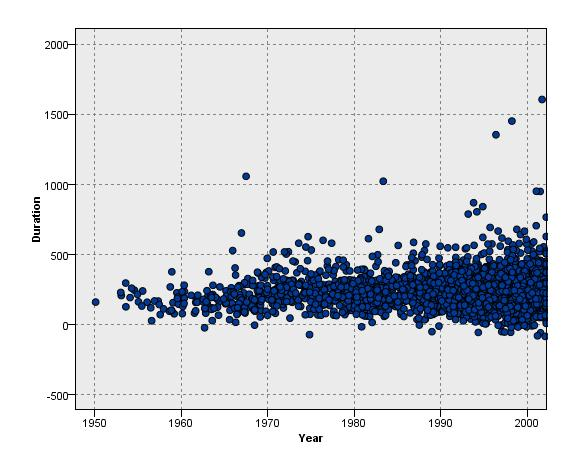
\includegraphics[scale=0.4]{resources/year-duration.jpg}
    \label{fig:YearDuration}
    \caption{Odnos godine i du\v{z}ine pesama}
\end{figure}
